\documentclass[12pt]{article}
\usepackage{amsmath}
\usepackage{fancyhdr}
\usepackage{hyperref}
\usepackage{graphicx}

\usepackage{mathtools}
\usepackage{pst-node}

\newcommand{\compactlist}{\setlength{\itemsep}{0pt} \setlength{\parskip}{0pt} \setlength{\leftskip}{-1em}}
\usepackage[top=0.9in, bottom=0.8in, left=0.9in, right=0.9in]{geometry}

\lhead{MATH 4363/5373}
\rhead{Sep. 25, 2019}
\chead[RE]{Lagrange interpolation}
\cfoot{}
%\rfoot{Code for figure and report is available in the class folder.}
\pagestyle{fancy}
\begin{document}
Below are \(L_k(x) = L_{7, k}(x)\) for \(8\) equally spaced points \(x_0 = -1, \dots, x_7 = 1\) on \([-1, 1]\). 

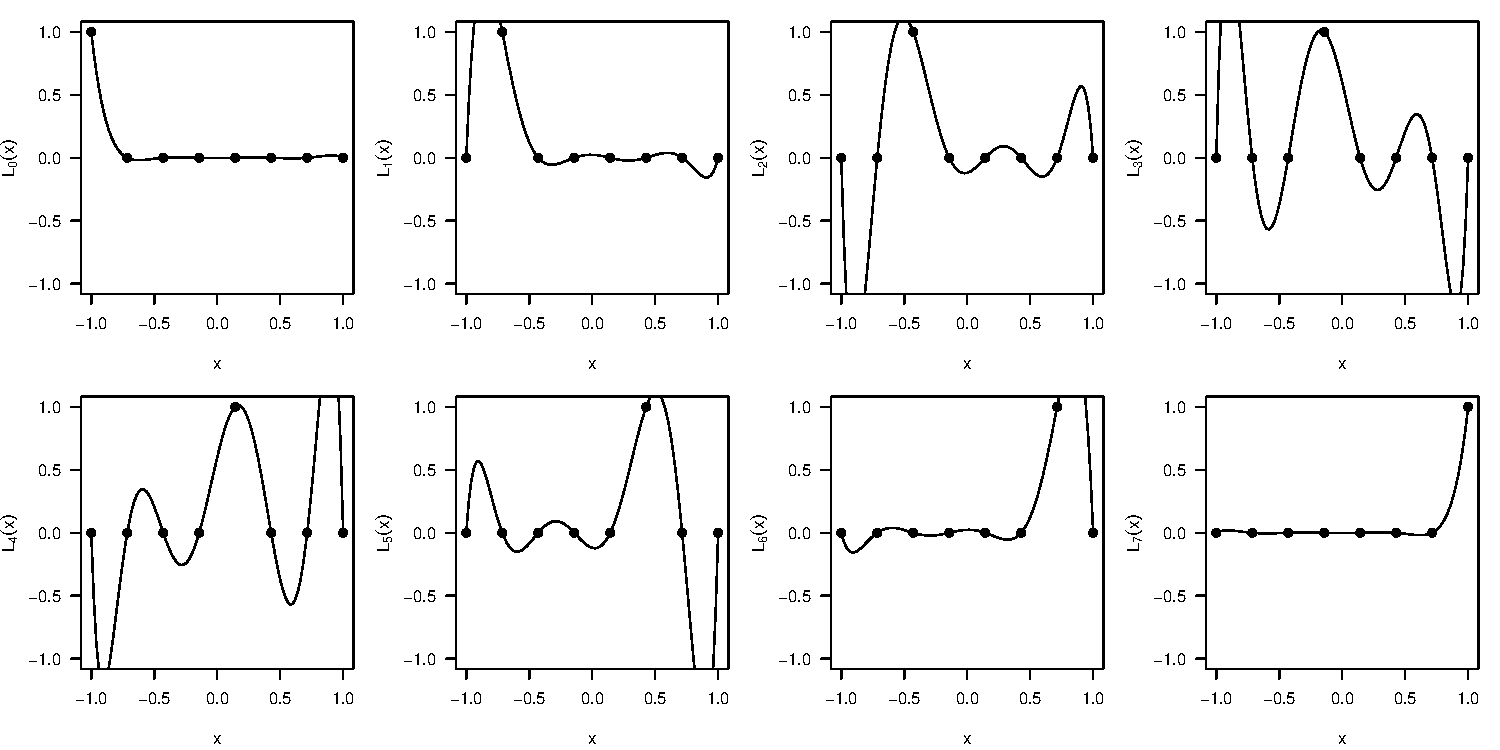
\includegraphics[width=\textwidth]{Li.pdf}

Considering the function \[f(x) = x^3e^{-1.1x}\sin(x)\] we show the approximation \[P(x) = P_7(x) = \sum_{k=0}^7 f(x_k)L_k(x)\] (along with the function) on the left and the error on the right.

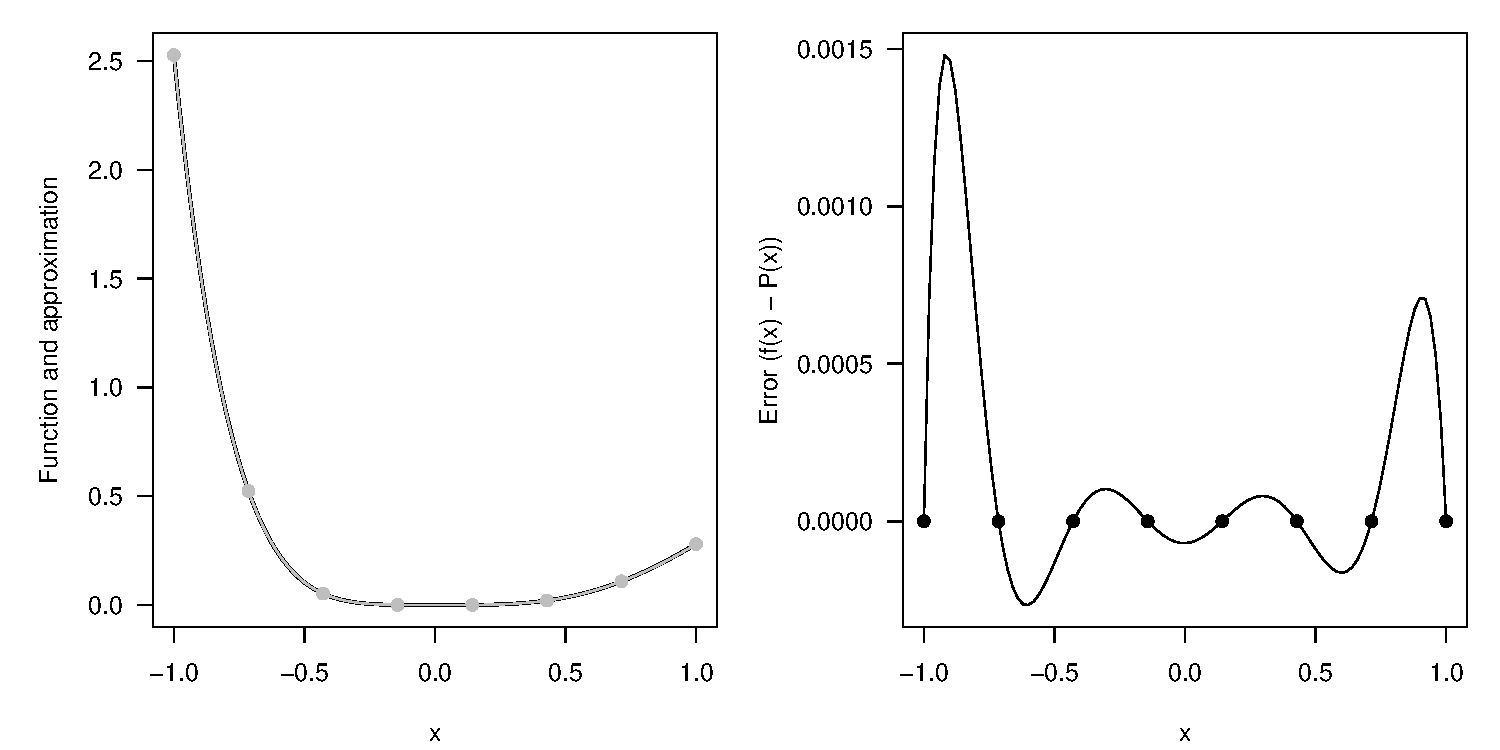
\includegraphics[width=\textwidth]{fP.pdf}

\end{document}